\documentclass[pdf,aspectratio=169,14pt]{beamer}
\mode<presentation>{}
\usepackage{listings}
\usepackage{graphicx}
\usepackage{theme/beamerthemecoreos169}
\usepackage{tikz}

\title{rktnetes}
\subtitle{Integrating rkt and Kubernetes}
\author{Derek Gonyeo, CoreOS}

\graphicspath{ {./images/} }

\usetikzlibrary{arrows,positioning} 
\tikzset{
    %Define standard arrow tip
    >=stealth',
    %Define style for boxes
    punkt/.style={
           rectangle,
           rounded corners,
           draw=white, very thick,
           text width=6.5em,
           minimum height=2em,
           text centered},
    % Define arrow style
    pil/.style={
           <->,
           thick,
           shorten <=2pt,
           shorten >=2pt,}
}

\newcommand{\mbold}[3]{
    \ifnum #1=#2
        \textbf{#3}
    \else
        #3
    \fi
}

\newcommand{\outline}[1]{
    \begin{frame}
        Outline
        \begin{itemize}
            \item \mbold{#1}{1}{What is rkt?}
            \item \mbold{#1}{2}{What is kubernetes?}
            \item \mbold{#1}{3}{What is rktnetes?}
            \item \mbold{#1}{4}{How does rktnetes work?}
            \item \mbold{#1}{5}{Why rktnetes?}
        \end{itemize}
    \end{frame}
}

\begin{document}

\begin{frame}
    \titlepage
\end{frame}

\begin{frame}{About Me}
    Derek Gonyeo \\
    rkt Scientist at CoreOS \\
    Student at RIT \\
    @dgonyeo
\end{frame}

\outline{0}

% Section: What is rkt?

\outline{1}

\begin{frame}{What is rkt?}
    rkt...
    \begin{itemize}
        \item<2-> is an open source project
        \item<3-> is a golang binary
        \item<4-> has a simple command line interface
        \item<5-> is packaged for CoreOS, Debian, Ubuntu, Fedora, Arch, Gentoo, and Nix
    \end{itemize}
\end{frame}

\begin{frame}{What is rkt?}
    rkt is a container runtime. \\
    \vspace{1em}
    This means that it will:
    \begin{itemize}
        \item<2-> Fetch container images
        \item<3-> Cryptographically verify container images
        \item<4-> Manage a local store of container images
        \item<5-> Run container images
        \item<6-> Provide information about running containers
    \end{itemize}
\end{frame}

\begin{frame}{What is rkt?}
    Notes on rkt's architecture:
    \begin{itemize}
        \item<2-> Has a pod-first design
        \item<3-> Does not have a central daemon
        \item<4-> Has swappable isolation models (more on this later)
    \end{itemize}
\end{frame}

\newcommand{\rktsection}[1]{
    \begin{frame}{What is rkt?}
        rkt is:
        \begin{itemize}
            \item \mbold{#1}{1}{Secure}
            \item \mbold{#1}{2}{Standards Compliant}
            \item \mbold{#1}{3}{Composable}
        \end{itemize}
    \end{frame}
}

% Subsection: secure

\rktsection{0}
\rktsection{1}

\begin{frame}{What is rkt?}
    How is rkt secure?
    \begin{itemize}
        \item<2-> Requires images to be GPG signed
        \item<3-> Uses selinux to prevent breakouts
        \item<4-> Uses seccomp to drop privileges
        \item<5-> Uses the TPM to make a tamper-proof audit log
        \item<6-> No central privileged daemon
    \end{itemize}
\end{frame}

\begin{frame}{What is rkt?}
    \center \includegraphics[width=0.75\textwidth]{rkt-vs-docker-fetch}
\end{frame}

% Subsection: standards compliant

\rktsection{1}
\rktsection{2}

\begin{frame}{What is rkt?}
    How is rkt standards compliant?
    \begin{itemize}
        \item<2-> Implementation of the AppC spec
        \item<3-> Supports images from the docker spec
        \item<4-> Supports images from the OCI spec
        \item<5-> Native OCI support coming
        \item<6-> Uses CNI for network configuration
    \end{itemize}
\end{frame}

% Subsection: composable

\rktsection{2}
\rktsection{3}

\begin{frame}{What is rkt?}
    How is rkt composable?
    \begin{itemize}
        \item<2-> Simple process model
        \item<3-> Swappable stage1s
        \item<4-> Systemd integration
    \end{itemize}
\end{frame}

\begin{frame}{What is rkt?}
    \center \includegraphics[width=0.75\textwidth]{rkt-vs-docker-process-model}
\end{frame}

\begin{frame}{What is rkt?}
    rkt has stages
\end{frame}

\begin{frame}{What is rkt?}
    stage0:
    \begin{itemize}
        \item<2-> Handles user interaction
        \item<3-> Fetches and verifies images
        \item<4-> Manages the image store
        \item<5-> Handles dependencies
        \item<6-> Renders images
        \item<7-> Execs stage1
    \end{itemize}
\end{frame}

\begin{frame}{What is rkt?}
    stage1:
    \begin{itemize}
        \item<2-> Sets up isolation for pod
        \item<3-> Sets up relevant networking
        \item<4-> Sets up mounts
        \item<5-> Execs stage2
    \end{itemize}
\end{frame}

\begin{frame}{What is rkt?}
    The stage2 is user provided - your app!
\end{frame}

\begin{frame}{What is rkt?}
    Available stage1s:
    \begin{itemize}
        \item<2-> coreos
        \item<3-> host
        \item<4-> fly
        \item<5-> kvm
    \end{itemize}
\end{frame}

\begin{frame}{What is rkt?}
    systemd isn't required to use rkt! \\
    \vspace{1em}
    \pause
    But if you are using systemd:
    \begin{itemize}
        \item<2-> Trivial to have rkt in systemd units
        \item<3-> journald integration
        \item<4-> machined integration
    \end{itemize}
\end{frame}

% Section: What is kubernetes?

\outline{1}
\outline{2}

\begin{frame}{What is kubernetes?}
    Kubernetes is:
    \begin{itemize}
        \item container orchestration
        \item cluster-level
        \item fault tolerant
    \end{itemize}
\end{frame}

\begin{frame}{What is kubernetes?}
    \begin{tikzpicture}[node distance=1cm, auto,]
     \node[punkt] (etcd) {etcd};
     \pause
     \node[punkt, inner sep=5pt,below=0.75cm of etcd] (kubeapi) {API Server}
       edge[pil] (etcd.south);
     \pause
     \node[punkt, inner sep=5pt,below=0.75cm of kubeapi] (kubelet0) {kubelet}
       edge[pil] (kubeapi.south);
     \node[punkt, inner sep=5pt,right=0.75cm of kubelet0] (kubelet1) {kubelet}
       edge[pil] (kubeapi.south);
     \node[punkt, inner sep=5pt,left=0.75cm of kubelet0] (kubelet2) {kubelet}
       edge[pil] (kubeapi.south);
    \end{tikzpicture}
\end{frame}

\begin{frame}{What is kubernetes?}
    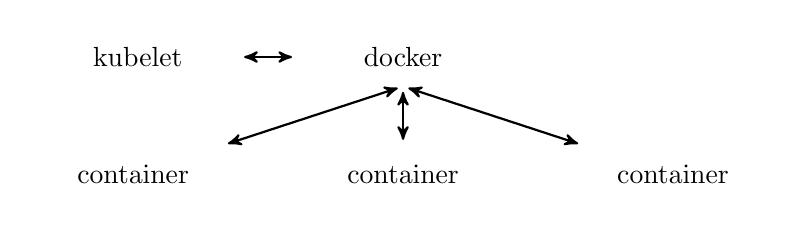
\begin{tikzpicture}[node distance=1cm, auto,]
     \node[punkt] (kubelet) {kubelet};
     \pause
     \node[punkt, inner sep=5pt,right=0.75cm of kubelet] (docker) {docker}
       edge[pil] (kubelet.east);
     \pause
     \node[punkt, inner sep=5pt,below=0.75cm of docker] (container0) {container}
       edge[pil] (docker.south);
     \node[punkt, inner sep=5pt,right=0.75cm of container0] (container1) {container}
       edge[pil] (docker.south);
     \node[punkt, inner sep=5pt,left=0.75cm of container0] (container2) {container}
       edge[pil] (docker.south);
    \end{tikzpicture}
\end{frame}

% Section: What is rktnetes?

\outline{2}
\outline{3}

\begin{frame}{What is rktnetes?}
    Use rkt as the container runtime!
\end{frame}

\begin{frame}{What is rktnetes?}
    Current status:
    \begin{itemize}
        \item<2-> Support included in Kubernetes 1.3
        \item<3-> >90\% of common end-to-end tests pass with rkt
        \item<4-> Still working on refining the integration
    \end{itemize}
\end{frame}

% Section: How does rktnetes work?

\outline{3}
\outline{4}

\begin{frame}{How does rktnetes work?}
    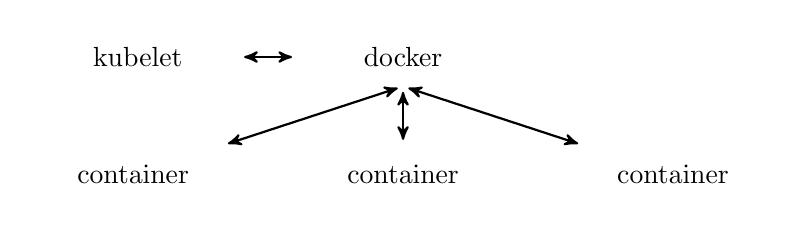
\begin{tikzpicture}[node distance=1cm, auto,]
     \node[punkt] (kubelet) {kubelet};
     \node[punkt, inner sep=5pt,right=0.75cm of kubelet] (docker) {docker}
       edge[pil] (kubelet.east);
     \node[punkt, inner sep=5pt,below=0.75cm of docker] (container0) {container}
       edge[pil] (docker.south);
     \node[punkt, inner sep=5pt,right=0.75cm of container0] (container1) {container}
       edge[pil] (docker.south);
     \node[punkt, inner sep=5pt,left=0.75cm of container0] (container2) {container}
       edge[pil] (docker.south);
    \end{tikzpicture}
\end{frame}

\begin{frame}{How does rktnetes work?}
    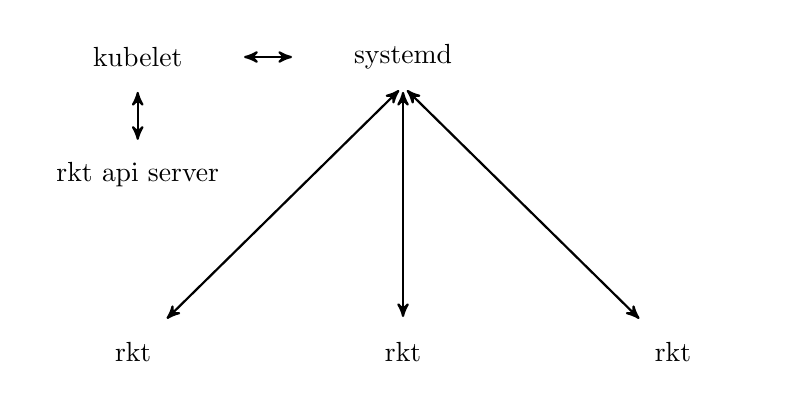
\begin{tikzpicture}[node distance=1cm, auto,]
     \node[punkt] (kubelet) {kubelet};
     \pause
     \node[punkt, inner sep=5pt,right=0.75cm of kubelet] (systemd) {systemd}
       edge[pil] (kubelet.east);
     \pause
     \node[punkt, inner sep=5pt,below=3cm of systemd] (container0) {rkt}
       edge[pil] (systemd.south);
     \node[punkt, inner sep=5pt,right=0.75cm of container0] (container1) {rkt}
       edge[pil] (systemd.south);
     \node[punkt, inner sep=5pt,left=0.75cm of container0] (container2) {rkt}
       edge[pil] (systemd.south);
     \pause
     \node[punkt, inner sep=5pt,below=0.75cm of kubelet] (rktapi) {rkt api server}
       edge[pil] (kubelet.south);
    \end{tikzpicture}
\end{frame}

\begin{frame}{How does rktnetes work?}
    rktnetes prerequisites:
    \begin{itemize}
        \item<2-> The host must use systemd
        \item<3-> rkt v1.9.1 or greater must be installed
        \item<4-> The rkt api service must be running
    \end{itemize}
\end{frame}

\begin{frame}{How does rktnetes work?}
    How do I use rktnetes?
    \begin{itemize}
        \item<2-> Add \texttt{-{}-container-runtime=rkt} to the kubelet
    \end{itemize}
\end{frame}

% Section: Why rktnetes?

\outline{4}
\outline{5}

\begin{frame}{Why rktnetes?}
    Why did we build this?
    \begin{itemize}
        \item Path to a generic container runtime interface
        \item rkt has a different feature set than docker
    \end{itemize}
\end{frame}

\begin{frame}
    \center \LARGE Questions?
    \normalsize
\end{frame}

\begin{frame}
    By the way: \\
    \vspace{1em}
    \pause
    \LARGE Kubernetes Community Bash \normalsize \\
    Tonight at 7 pm \\
    Real Sports Bar \& Grill \\
    \vspace{1em}
    https://kubernetesecosystembash.eventbrite.com/
\end{frame}

\end{document}
